\section{Questpackage}
%TODO referenz folgt Quest Package erklärung
Hier kann man zwischen den vorhanden Quest Packages (siehe Kapitel \ref{sec:Package}) wählen, wobei rechts die Beschreibung des jeweiligen Packages, falls diese vorhanden ist, angezeigt wird. Mithilfe eines Klicks auf den Pfeil kann das gewünschte Package ausgewählt werden.

\begin{figure}[h] 
  \centering
     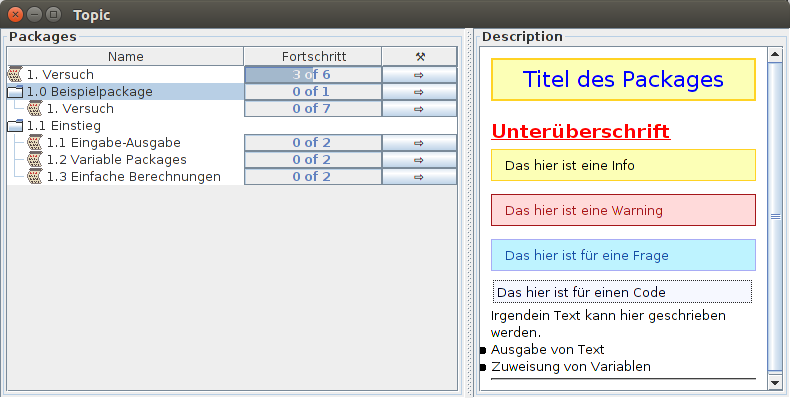
\includegraphics[width=1\textwidth]{./media/images/gui/package-auswahl.png}
  \caption{Auswahl des Packages}
  \label{fig:Package_Auswahl}
\end{figure}

Weiters wird auch der Fortschritt des Packages angezeigt. Daraus ist ersichtlich, wie viele Quests man in dem Packet bereits fertiggestellt hat.

Bei einem Quest Package wurde eine JTreeTable (siehe Kapitel: \ref{}) zur Realisierung verwendet. Diese befindet sich wiederum in einer JScrollpane. Somit ist die Anzahl der Elemente in der JTable\footnote{\url{https://docs.oracle.com/javase/tutorial/uiswing/components/scrollpane.html}}  und der JTreeTable nicht begrenzt.
